\whiteBGstarBegin
\begin{enumerate}[label=\bfseries Câu \arabic*:]
	
	\item \mkstar{1}
	
	\cauhoi
	{Chuyển động thẳng đều là
		\begin{mcq}
			\item chuyển động thẳng, trong đó chất điểm có gia tốc không đổi.
			\item chuyển động có quỹ đạo là đường thẳng và có gia tốc như nhau trên mọi quãng đường.
			\item chuyển động có quỹ đạo là đường thẳng và có tốc độ trung bình như nhau trên mọi quãng đường.
			\item chuyển động thẳng, trong đó chất điểm có vận tốc tức thời thay đổi.
		\end{mcq}
	}
	
	\loigiai
	{\textbf{Đáp án: C.}
		
		Chuyển động thẳng đều là chuyển động có quỹ đạo là đường thẳng và có tốc độ trung bình như nhau trên mọi quãng đường.
		
		
	}
	\item \mkstar{1}
	
	\cauhoi
	{Phương trình chuyển động của chuyển động thẳng chậm dần đều là
		\begin{mcq}
			\item $x=x_0+v_0t +\dfrac{at^2}{2}$ ($a$ và $v_0$ trái dấu).
			\item $s=v_0t+\dfrac{at^2}{2}$ ($a$ và $v_0$ trái dấu).
			\item $x=x_0+v_0t +\dfrac{at^2}{2}$ ($a$ và $v_0$ cùng dấu).
			\item $s=v_0t+\dfrac{at^2}{2}$ ($a$ và $v_0$ cùng dấu).
		\end{mcq}
	}
	\loigiai
	{\textbf{Đáp án: A.}
		
		Phương trình chuyển động của chuyển động thẳng chậm dần đều là
		$$x=x_0+v_0t +\dfrac{at^2}{2}\ (a \textrm{ và } v_0 \text{ trái dấu}).$$
		
		
	}
	\item \mkstar{1}
	
	\cauhoi
	{Chỉ ra câu \textbf{sai}.
		\begin{mcq}
			\item Gia tốc của chuyển động thẳng biến đổi đều có độ lớn không đổi. 
			\item Trong chuyển động thẳng biến đổi đều, quãng đường đi được trong những khoảng thời gian bằng nhau thì bằng nhau.
			\item Vận tốc tức thời của chuyển động thẳng biến đổi đều có độ lớn tăng hoặc giảm đều theo thời gian.
			\item Vectơ gia tốc của chuyển động thẳng biến đổi đều có thể cùng chiều hoặc ngược chiều với vectơ vận tốc.
		\end{mcq}
		
	}
	\loigiai
	{\textbf{Đáp án: B.}
		
		Công thức tính quãng đường đi được trong chuyển động thẳng biến đổi đều là
		$$s=v_0t+\dfrac{1}{2}at^2=\dfrac{1}{2}\left(v_0 + v_0+at \right) t=\dfrac{1}{2}\left(v_0+v\right) t\ (\text{với } v=v_0+at).$$
		
		Trong chuyển động biến đổi đều vận tốc $v$ thay đổi sau những khoảng thời gian bằng nhau, nên quãng đường đi được $s$ cũng thay đổi sau những khoảng thời gian bằng nhau.
		
		
	}
	\item \mkstar{2}
	
	\cauhoi
	{Phương trình chuyển động thẳng đều của một chất điểm có dạng $x=-4t+12$\\ ($x$: km, $t$: h). Quãng đường của chất điểm đi được sau $\SI{2}{\hour}$ là
		\begin{mcq}(4)
			\item $\SI{6}{\kilo\meter}$.
			\item $\SI{8}{\kilo\meter}$.
			\item $\SI{2}{\kilo\meter}$.
			\item $\SI{4}{\kilo\meter}$.
		\end{mcq}
	}
	\loigiai
	{\textbf{Đáp án: B.}	
		
		Quãng đường của chất điểm đi được sau $\SI{2}{\hour}$ là
		$$s=v_0t=\SI{4}{\kilo\meter/\hour}\cdot\SI{2}{\hour}=\SI{8}{\kilo\meter}.$$
		
		
	}
	\item \mkstar{2}
	
	\cauhoi
	{Một ôtô chuyển động trên một đoạn đường thẳng với tốc độ $\SI{60}{\kilo\meter/\hour}$. Bến xe nằm ở đầu đoạn đường nhưng xe xuất phát từ một điểm trên đoạn đường cách bến xe $\SI{4}{\kilo\meter}$. Chọn bến xe là vật mốc, chọn thời điểm xe xuất phát làm gốc thời gian và chọn chiều dương là chiều chuyển động. Phương trình chuyển động của ôtô trên đoạn đường này là
		\begin{mcq}(2)
			\item $x=60t$ (km, h).
			\item $x=4-60t$ (km, h).
			\item $x=4+60t$ (km, h).
			\item $x=-4-60t$ (km, h).
		\end{mcq}
		
	}
	\loigiai
	{\textbf{Đáp án: C.}
		
		Chọn bến xe là vật mốc, chọn thời điểm xe xuất phát làm gốc thời gian và chọn chiều dương là chiều chuyển động nên $x_0=\SI{4}{\kilo\meter}$, $v_0=\SI{60}{\kilo\meter/\hour}$.
		
		Phương trình chuyển động của ôtô trên đoạn đường này là: $x=4+60t$ (km, h).
		
		
	}
	\item \mkstar{2}
	
	\cauhoi{
		Trên trục $\text O x$ có hai ô tô chuyển động với phương trình tọa độ lần lượt là $x_1 (t) = -20t+100\ (\text {m; s})$ và $x_2 (t) = 10t-50\ (\text {m; s})$. Khoảng cách giữa hai ô tô lúc $t=2\ \text s$ là
		\begin{mcq}(4)
			\item $\SI{90}{\meter}$.
			\item $\SI{0}{\meter}$.
			\item $\SI{60}{\meter}$.
			\item $\SI{30}{\meter}$.
		\end{mcq}
	}
	\loigiai
	{\textbf{Đáp án: A.}
		
		Tại thời điểm $t=2\ \text s$ thì các ô tô có tọa độ là $x_1 = \SI{60}{\meter}$, $x_2 = \SI{-30}{\meter}$.
		
		Khoảng cách giữa hai ô tô lúc $t=2\ \text s$ là $\SI{90}{\meter}$.
		
		
	}
	\item \mkstar{2}
	
	\cauhoi{
		Lúc 7 giờ, một người ở A chuyển động thẳng đều với vận tốc $v=\SI{36}{\kilo \meter / \hour}$ đuổi theo người ở B đang chuyển động với vận tốc $v=\SI{5}{\meter / \second}$. Biết $\text{AB}=\SI{18}{\kilo \meter}$. Chọn gốc tọa độ ở A, chiều dương là chiều chuyển động. Phương trình chuyển động của người A và B lần lượt là
		\begin{mcq}(1)
			\item $x_\text A = 36t +18\ \text{(km, h)}$; $x_\text B = 18t\ \text{(km, h)}$.
			\item $x_\text A = 36t -18\ \text{(km, h)}$; $x_\text B = 18t + 18\ \text{(km, h)}$.
			\item $x_\text A = 36t\ \text{(km, h)}$; $x_\text B = 18t+18\ \text{(km, h)}$.
			\item $x_\text A = 36t\ \text{(km, h)}$; $x_\text B = 18t\ \text{(km, h)}$.
		\end{mcq}	
	}
	\loigiai
	{\textbf{Đáp án: C.}
		
		 Chọn gốc tọa độ ở A, chiều dương là chiều chuyển động.
		
		Phương trình chuyển động của người ở A: $x_\text A = 36t+0=36t\ \text{(km, h)}$.
		
		Phương trình chuyển động của người ở B (đổi $\SI{5}{\meter / \second} \rightarrow \SI{18}{\kilo \meter / \hour}$): $x_\text B = 18t+18\ \text{(km, h)} $.
		
		
	}
	\item \mkstar{2}
	
	\cauhoi{ Phương trình chuyển động của một vật trên một đường thẳng có dạng $x=2t^2 + 10t+100\ \text{(m; s)}$. Thông tin nào sau đây là đúng?
		\begin{mcq}(1)
			\item Vật chuyển động nhanh dần đều với gia tốc là $a=\SI{2}{\meter / \second \squared}$.
			\item Vật chuyển động chậm dần đều với gia tốc là $a=\SI{4}{\meter / \second \squared}$.
			\item Tọa độ của vật lúc $t=\SI{0}{\second}$ là $x=\SI{100}{\meter}$.
			\item Vận tốc của vật tại mọi thời điểm là $v=\SI{10}{\meter / \second}$.
		\end{mcq}
	}
	\loigiai
	{\textbf{Đáp án: C.}
		
		
		Phương trình chuyển động thẳng biến đổi đều: $x=\dfrac{1}{2}at^2+v_0t+x_0$.
		
		Ta thấy $a=\SI{4}{\meter / \second \squared}$, $v_0=\SI{10}{\meter / \second}$, $x_0=\SI{100}{\meter}$.
		
		Do $a$ và $v_0$ cùng dấu nên vật chuyển động nhanh dần đều với gia tốc $a=\SI{4}{\meter / \second \squared}$, thời điểm ban đầu ($t=\SI{0}{\second}$) vật có tọa độ $x=\SI{100}{\meter}$.
		
		
	}
	\item \mkstar{2}
	
	\cauhoi{Phương trình chuyển động của một vật trên một đường thẳng có dạng $x=4t^2-3t+3\ \text{(m; s)}$. Điều nào sau đây đúng?
		\begin{mcq}(1)
			\item Gia tốc của vật là $a=\SI{4}{\meter / \second \squared}$.
			\item Tọa độ của vật ở thời điểm ban đầu là $x_0=\SI{6}{\meter}$.
			\item Tọa độ của vật ở thời điểm $\SI{1}{\second}$ là $x=\SI{3}{\meter}$.
			\item Vận tốc ban đầu của vật là $v_0=\SI{-3}{\meter / \second}$.
		\end{mcq}
	}
	\loigiai
	{\textbf{Đáp án: D.}
		
		Phương trình chuyển động thẳng biến đổi đều: $x=\dfrac{1}{2}at^2+v_0t+x_0$.
		
		Ta thấy $a=\SI{8}{\meter / \second \squared}$, $v_0=\SI{-3}{\meter / \second}$, $x_0=\SI{3}{\meter}$.
		
		
	}
	\item \mkstar{2}
	
	\cauhoi{Một vật chuyển động thẳng chậm dần đều với tốc độ ban đầu $\SI{3}{\meter/\second}$ và gia tốc có độ lớn $\SI{2}{\meter/\second^2}$. Biết thời điểm ban đầu vật ở gốc tọa độ và chuyển động ngược chiều dương của trục tọa độ. Phương trình chuyển động của vật là
		\begin{mcq}(2)
			\item $x=-3t-t^2$ (m, s).
			\item $x=3t+t^2$ (m, s).
			\item $x=-3t-t^2$ (m, s).
			\item $x=-3t+t^2$ (m, s).
		\end{mcq}
	}
	\loigiai
	{\textbf{Đáp án: D.}
		
		Chọn gốc thời gian là khi vật bắt đầu chuyển động.
		
		Vì vật chuyển động chậm dần đều ngược chiều dương nên:
		\begin{equation*}
			\left\{\begin{array}{ll}{a\cdot v <0}&\\{v < 0}&\end{array}\right.\Rightarrow \left\{\begin{array}{ll}{a > 0}&\\{v < 0.}&\end{array}\right.
		\end{equation*}
		
		Kết hợp với các dữ kiện của đề bài, ta suy ra:
		\begin{equation*}
			\left\{\begin{array}{ll}{a=\SI{2}{\meter/\second^2}}&\\{v=\SI{-3}{\meter/\second} .}&\end{array}\right.
		\end{equation*}
		
		Phương trình chuyển động của vật có dạng:
		$x=-3t+t^2$ (m, s).
		
		
	}
	\item \mkstar{2}
	
	\cauhoi{Lúc $\SI{7}{\hour}$, hai ô tô bắt đầu khởi hành từ hai điểm A, B cách nhau $\SI{2400}{\meter}$, chuyển động nhanh dần đều và ngược chiều nhau. Ô tô đi từ A có gia tốc $\SI{1}{\meter / \second \squared}$, còn ô tô đi từ B có gia tốc $\SI{2}{\meter / \second \squared}$. Chọn chiều dương hướng từ A đến B, gốc thời gian lúc $\SI{7}{\hour}$. Xác định vị trí hai xe gặp nhau.
		\begin{mcq}(4)
			\item $\SI{1600}{\meter}$.
			\item $\SI{1200}{\meter}$.
			\item $\SI{800}{\meter}$.
			\item $\SI{2400}{\meter}$.
		\end{mcq}
	}
	\loigiai
	{\textbf{Đáp án: C.}
		
		Chọn chiều dương hướng từ A đến B, gốc thời gian lúc $\SI{7}{\hour}$.
		
		Phương trình chuyển động của xe A: $x_\text A = 0,5t^2$.
		
		Phương trình chuyển động của xe B: $x_\text B=-t^2 + 2400$.
		
		Hai xe gặp nhau: $x_\text A = x_\text B \Rightarrow t = \SI{40}{\second} \Rightarrow x=\SI{800}{\meter}$.
		
		
	}
	\item \mkstar{3}
	
	\cauhoi{Một xe chạy trong $\SI{5}{\hour}$, $\SI{2}{\hour}$ đầu xe chạy với tốc độ trung bình $\SI{60}{\km/\hour}$, $\SI{3}{\hour}$ sau xe chạy với tốc độ trung bình $\SI{40}{\km/\hour}$. Tốc độ trung bình của xe trong suốt thời gian chuyển động là
		\begin{mcq}(4)
			\item $\SI{48}{\kilo\meter/ \hour}$.
			\item $\SI{36}{\kilo\meter/ \hour}$.
			\item $\SI{54}{\kilo\meter/ \hour}$.
			\item $\SI{72}{\kilo\meter/ \hour}$.
		\end{mcq}
	}
	\loigiai
	{\textbf{Đáp án: A.}
		
		Quãng đường đi trong $\SI{2}{\hour}$ đầu là
		$$s_1 = v_1t_1 = \SI{60}{\km/\hour}\cdot\SI{2}{\hour} = \SI{120}{km}.$$
		Quãng đường đi trong $\SI{3}{\hour}$ sau là
		$$s_2 = v_2t_2 = \SI{40}{\km/\hour}\cdot\SI{3}{\hour} = \SI{120}{km}.$$
		Tốc độ trung bình của xe trong suốt thời gian chuyển động là
		$$v_{\text{tb}}=\dfrac{s_1+s_2}{t_1+t_2}=\dfrac{\SI{120}{km}+\SI{120}{km}}{\SI{2}{\hour}+\SI{3}{\hour}}=\SI{48}{\km/\hour}.$$
		
		
	}
	\item \mkstar{3}
	
	\cauhoi{ Vật chuyển động thẳng đều có đồ thị tọa độ - thời gian như hình vẽ. Phương trình chuyển động của vật có dạng nào sau đây?
		\begin{center}
			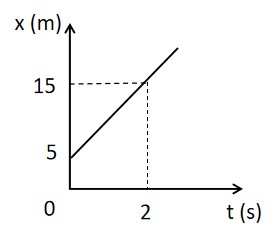
\includegraphics[scale=0.9]{../figs/VN11-Y21-PH-SYL-001-1.jpg}
		\end{center}
		\begin{mcq}(4)
			\item $x=5+5t$.
			\item $x=4t$.
			\item $x=5-5t$.
			\item $x=5+4t$.
		\end{mcq}
	}
	\loigiai
	{\textbf{Đáp án: A.}
		
		Vận tốc của vật là
		\begin{equation*}
			v=\dfrac{x-x_0}{t-t_0}=\dfrac{\SI{15}{\meter}-\SI{5}{\meter}}{\SI{2}{\second}}=\SI{5}{\meter/\second}.
		\end{equation*}
		
		Phương trình chuyển động của vật là
		\begin{equation*}
			x=x_0+vt=5+5t\textrm{ (m, s)}.
		\end{equation*}
		
		
	}
	\item \mkstar{3}
	
	\cauhoi{Khi ô tô đang chạy với vận tốc $\SI{10}{\meter/\second}$ trên đoạn đường thẳng thì người lái xe tăng ga và ô tô chuyển động nhanh dần đều. Sau $\SI{20}{\second}$, ô tô đạt vận tốc $\SI{14}{\meter/\second}$. Gia tốc $a$ và vận tốc $v$ của ô tô sau $\SI{40}{\second}$ kể từ lúc bắt đầu tăng ga là bao nhiêu?
		\begin{mcq}(2)
			\item $a=\SI{0.2}{\meter/\second}^2$; $v=\SI{18}{\meter/\second}$.
			\item $a=\SI{0.2}{\meter/\second}^2$; $v=\SI{8}{\meter/\second}$.
			\item $a=\SI{0.7}{\meter/\second}^2$; $v=\SI{38}{\meter/\second}$.
			\item $a=\SI{1.4}{\meter/\second}^2$; $v=\SI{66}{\meter/\second}$.
		\end{mcq}
	}
	\loigiai
	{\textbf{Đáp án: A.}
		
		Gia tốc của ô tô:
		$$a=\dfrac{v-v_0}{t}=\dfrac{\SI{14}{\meter/\second}-\SI{10}{\meter/\second}}{\SI{20}{\second}}=\SI{0.2}{\meter/\second^2}.$$
		Vận tốc của ô tô:
		$$v=v_0+at=\SI{10}{\meter/\second}+\SI{0.2}{\meter/\second^2}\cdot\SI{40}{\second}=\SI{18}{\meter/\second}.$$
		
		
	}
	\item \mkstar{3}
	
	\cauhoi{ Một vật chuyển động thẳng chậm dần đều với tốc độ ban đầu $\SI{4}{\meter/\second}$ và gia tốc có độ lớn $\SI{2}{\meter/\second^2}$. Biết thời điểm ban đầu vật ở gốc tọa độ và chuyển động cùng chiều dương của trục tọa độ. Phương trình chuyển động của vật là
		\begin{mcq}(2)
			\item $x=-4t-t^2$ (m, s).
			\item $x=4t-t^2$ (m, s).
			\item $x=4t-t^2$ (m, s).
			\item $x=-4t+t^2$ (m, s).
		\end{mcq}
	}
	\loigiai
	{\textbf{Đáp án: B.}
		
		Chọn gốc thời gian là khi vật bắt đầu chuyển động.
		
		Vì vật chuyển động chậm dần đều cùng chiều dương nên:
		\begin{equation*}
			\left\{\begin{array}{ll}{a\cdot v <0}&\\{v > 0}&\end{array}\right.\Rightarrow \left\{\begin{array}{ll}{a < 0}&\\{v > 0.}&\end{array}\right.
		\end{equation*}
		
		Kết hợp với các dữ kiện của đề bài, ta suy ra:
		\begin{equation*}
			\left\{\begin{array}{ll}{a=\SI{-2}{\meter/\second^2}}&\\{v=\SI{4}{\meter/\second} .}&\end{array}\right.
		\end{equation*}
		
		Phương trình chuyển động của vật có dạng:
		$x=4t-t^2$ (m, s).
		
		
	}
	\item \mkstar{3}
	
	\cauhoi{Một vật bắt đầu chuyển động từ trạng thái nghỉ với gia tốc không đổi $\SI{5}{\meter / \second \squared}$ trong $\SI{8}{\second}$. Sau thời gian này, vật chuyển động đều. Quãng đường vật đã đi được trong $\SI{12}{\second}$ kể từ lúc vật bắt đầu chuyển động là
		\begin{mcq}(4)
			\item $\SI{160}{\meter}$.
			\item $\SI{320}{\meter}$.
			\item $\SI{360}{\meter}$.
			\item $\SI{40}{\meter}$.
		\end{mcq}
	}
	\loigiai
	{\textbf{Đáp án: B.}
		
		Quãng đường vật đi được trong $\SI{8}{\second}$ đầu: $s_1=\dfrac{1}{2}at^2=\SI{160}{\meter}$.
		
		Vận tốc của vật ở cuối giây thứ 8: $v=at=\SI{40}{\meter / \second}$.
		
		Quãng đường vật đi được trong $\SI{4}{\second}$ sau:
		$s_2=vt=\SI{160}{\meter}$.
		
		Tổng quãng đường vật đã đi được trong $\SI{12}{\second}$ kể từ lúc vật bắt đầu chuyển động: $$s=s_1+s_2=\SI{320}{\meter}.$$
		
	}
	\item \mkstar{3}
	
	\cauhoi{Một ô tô đi từ A đến B. Đầu chặng ô tô đi 1/4 tổng thời gian với $v_1=\SI{50}{\km/\hour}$. Giữa chặng ô tô đi 1/2 tổng thời gian với $v_2=\SI{40}{\km/\hour}$. Cuối chặng ô tô đi 1/4 tổng thời gian với $v_3=\SI{20}{\km/\hour}$. Tốc độ trung bình của ô tô là
		\begin{mcq}(4)
			\item $\SI{37,5}{\kilo\meter/\hour}$.
			\item $\SI{50,2}{\kilo\meter/\hour}$.
			\item $\SI{70}{\kilo\meter/\hour}$.
			\item $\SI{85}{\kilo\meter/\hour}$.
		\end{mcq}
	}
	\loigiai
	{	\textbf{Đáp án: A.}
		
		Quãng đường ô tô đi đầu chặng là
		$$s_1=v_1t_1=v_1\cdot\dfrac{t}{4}.$$
		Quãng đường ô tô đi giữa chặng là
		$$s_2=v_2t_2=v_2\cdot\dfrac{t}{2}.$$
		Quãng đường ô tô đi cuối chặng là
		$$s_3=v_3t_3=v_3\cdot\dfrac{t}{4}.$$
		Tốc độ trung bình của ô tô là
		$$v_{\text{tb}}=\dfrac{s_1+s_2+s_3}{t}=\dfrac{v_1\cdot\dfrac{t}{4}+v_2\cdot\dfrac{t}{2}+v_3\cdot\dfrac{t}{4}}{t}=\dfrac{v_1}{4}+\dfrac{v_2}{2}+\dfrac{v_3}{4}=\SI{37,5}{\km/\hour}.$$
		
	
	}
	\item \mkstar{4}
	
	\cauhoi{Một người đang đi xe máy với vận tốc $\SI{36}{\kilo\meter/\hour}$ thì nhìn thấy chướng ngại vật cách đó $\SI{10}{\meter}$. Biết khối lượng tổng cộng của người và xe máy là $\SI{130}{\kilogram}$. Coi chuyển động của xe là chuyển động thẳng biến đổi đều sau khi hãm. Để không đâm phải chướng ngại vật thì vật phải có gia tốc nhỏ nhất là bao nhiêu?
		\begin{mcq}(4)
			\item $\SI{-5}{\meter/\second^2}$.
			\item $\SI{5}{\meter/\second^2}$.
			\item $\SI{-10}{\meter/\second^2}$.
			\item $\SI{10}{\meter/\second^2}$.
		\end{mcq}
		
	}
	\loigiai
	{\textbf{Đáp án: A.}
		
		Gia tốc nhỏ nhất để xe máy kịp dừng lại trước chướng ngại vật là:
		$$v^2-v_0^2=2a_\text{min} s\Rightarrow 0^2-(\SI{10}{\meter/\second})^2=2\cdot a_\text{min} \cdot \SI{10}{\meter}\Rightarrow a_\text{min}=\SI{-5}{\meter/\second^2}.$$
		
		
	}
	\item \mkstar{4}
	
	\cauhoi{ Một ôtô chạy đều trên một con đường thẳng với tốc độ $\SI{25}{\meter/\second}$ (vượt quá tốc độ) thì bị cảnh sát giao thông phát hiện. Chỉ sau $\SI{2}{\second}$ khi ôtô đi qua một cảnh sát, anh cảnh sát này bắt đầu đuổi theo với gia tốc không đổi và bằng $\SI{6}{\meter/\second^2}$. Thời điểm và vị trí anh cảnh sát đuổi kịp ôtô là
		\begin{mcq}
			\item sau $\SI{1}{\second}$ kể từ lúc anh cảnh sát xuất phát, cách vị trí xuất phát của anh cảnh sát $\SI{75}{\meter}$.
			\item  sau $\SI{10}{\second}$ kể từ lúc anh cảnh sát xuất phát, cách vị trí xuất phát của anh cảnh sát $\SI{300}{\meter}$.
			\item sau $\SI{12}{\second}$ kể từ lúc anh cảnh sát xuất phát, cách vị trí xuất phát của anh cảnh sát $\SI{300}{\meter}$.
			\item sau $\SI{3}{\second}$ kể từ lúc anh cảnh sát xuất phát, cách vị trí xuất phát của anh cảnh sát $\SI{75}{\meter}$.
		\end{mcq}
	}
	\loigiai
	{\textbf{Đáp án: B.}
		
		Chọn chiều dương là chiều chuyển động của xe ôtô và anh cảnh sát, gốc tọa tọa là vị trí của anh cảnh sát đang đứng, gốc thời gian là thời điểm cảnh sát bắt đầu đuổi theo xe.
		
		Phương trình chuyển động của xe ôtô là
		$$x=x_0+v_0(t+2)=25(t+2)\ \text{(m; s)}.$$
		
		Phương trình chuyển động của anh cảnh sát là
		$$x'=x_0'+v_0't+\dfrac{1}{2}at^2=3t^2\ \text{(m; s)}.$$
		
		Thời điểm anh cảnh sát đuổi kịp xe ôtô là
		$$x=x'\Rightarrow 25(t+2)=3t^2\Rightarrow t=\SI{10}{\second}.$$
		
		Vị trí anh cảnh sát đuổi kịp xe ôtô là
		$$x'=3t^2=\SI{300}{\meter}.$$
		
		
	}
	\item \mkstar{4}
	
	\cauhoi{Hai chất điểm A và B cách nhau $\SI{60}{\meter}$. Tại thời điểm $t=0$ chất điểm A chuyển động về phía B với vận tốc không đổi $\SI{12}{\meter / \second}$. Cùng thời điểm đó chất điểm B cũng chuyển động với gia tốc $\SI{2}{\meter / \second \squared}$ theo hướng ra xa A. Khoảng cách giữa A và B ngắn nhất tại thời điểm
		\begin{mcq}(4)
			\item $t=\SI{4}{\second}$.
			\item $t=\SI{5}{\second}$.
			\item $t=\SI{6}{\second}$.
			\item $t=\SI{2}{\second}$.
		\end{mcq}
	}
	\loigiai
	{\textbf{Đáp án: C.}
		
		Chọn chiều dương của trục $\text O x$ cùng hướng chuyển động của A và B, gốc O tại vị trí ban đầu của A. Gốc thời gian là lúc vật A và B bắt đầu chuyển động.
		
		Phương trình chuyển động của A: $x_\text A = 12t$.
		
		Phương trình chuyển động của B: $x_\text B = t^2 + 60$.
		
		Khoảng cách giữa A và B: $|x_\text B - x_\text A |=|t^2+60-12t|=|(t-6)^2+24|$.
		
		Khoảng cách này nhỏ nhất khi $(t-6)^2 = 0 \Rightarrow t=\SI{6}{\second}$.
		
		
	}
\end{enumerate}

\whiteBGstarEnd

\loigiai{\begin{center}
		\textbf{BẢNG ĐÁP ÁN}
	\end{center}
	\begin{center}
		\begin{tabular}{|m{2.8em}|m{2.8em}|m{2.8em}|m{2.8em}|m{2.8em}|m{2.8em}|m{2.8em}|m{2.8em}|m{2.8em}|m{2.8em}|}
			\hline
			1.C  & 2.A  & 3.B  & 4.B  & 5.C  & 6.A  & 7.C  & 8.C  & 9.D  & 10.D  \\
			\hline
			11.C  & 12.A  & 13.A  & 14.A  & 15.B  & 16.B  & 17.A  & 18.A  & 19.B  & 20.C  \\
			\hline
			
		\end{tabular}
\end{center}}